\chapter{Исследовательская часть}

\section{Среда для тестирования}

Для тестирования разработанного алгоритма применялась облачная платформа Google Colab, не требующая установки ПО на локальный компьютер.

% 

\section{Обучение модели полиномиальной регрессии}

\begin{figure}
	\begin{center}
		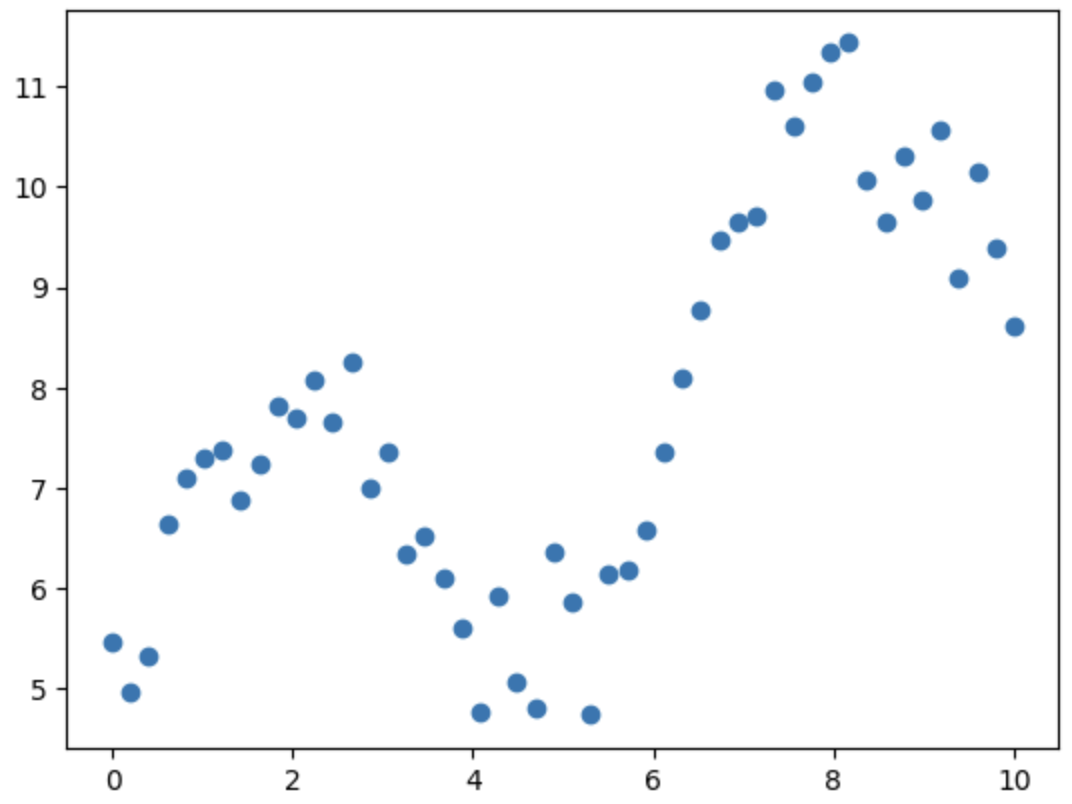
\includegraphics[width=0.75\textwidth]{images/1.png}
	\end{center}
	\caption{Исходные данные}
	\label{img:1}
\end{figure}

\begin{figure}
	\begin{center}
		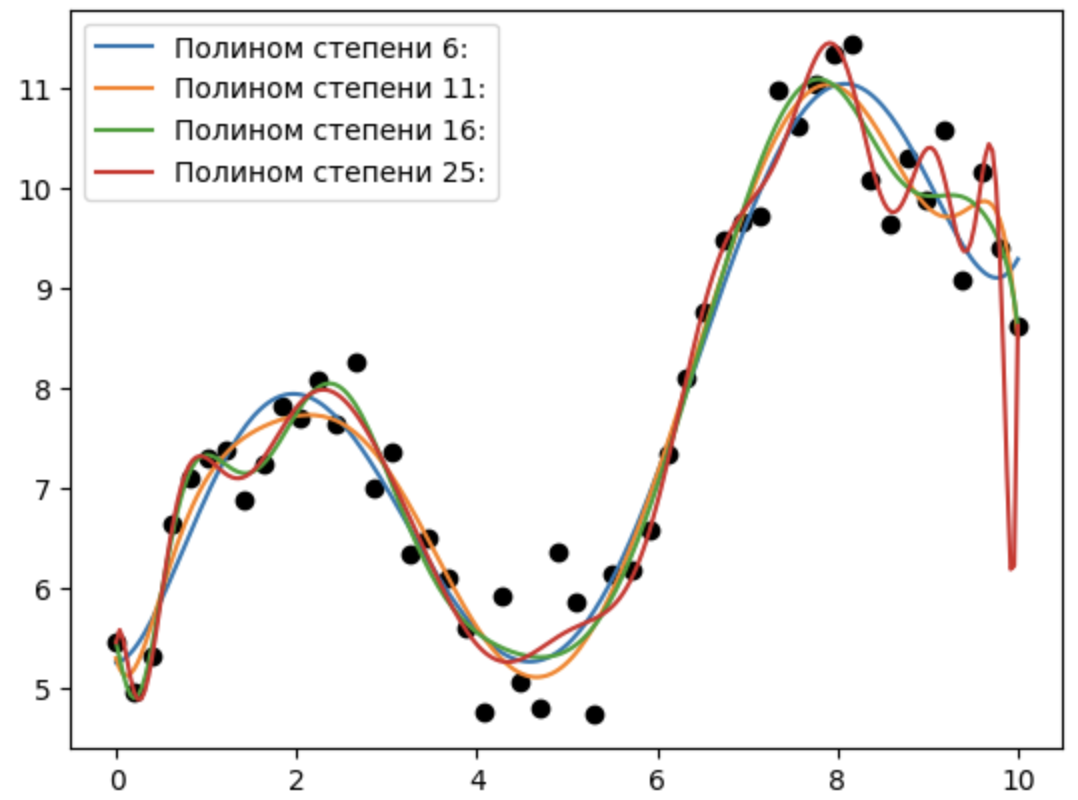
\includegraphics[width=0.75\textwidth]{images/2.png}
	\end{center}
	\caption{Аппроксимация полиномами различных степеней}
	\label{img:2}
\end{figure}

\begin{figure}
	\begin{center}
		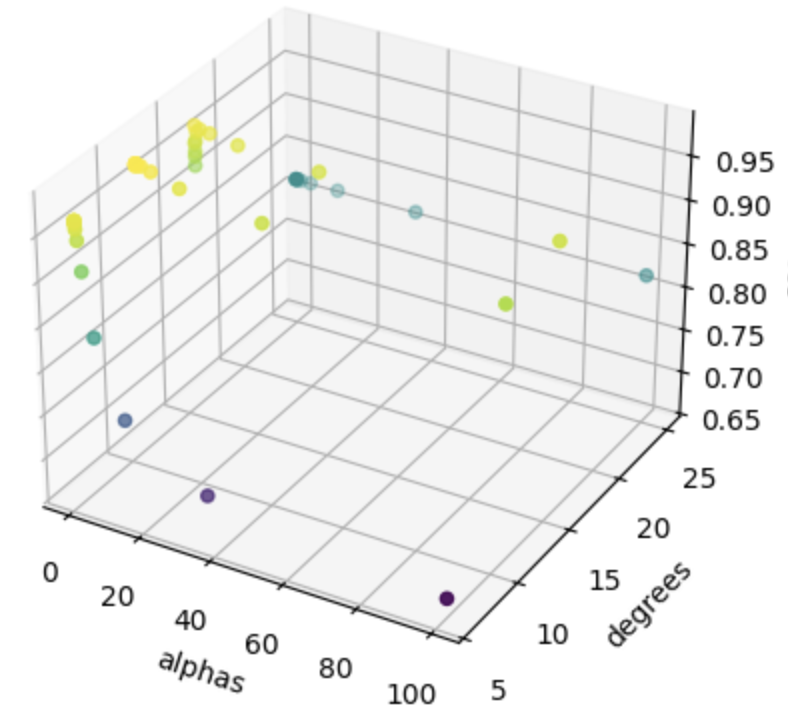
\includegraphics[width=0.75\textwidth]{images/3.png}
	\end{center}
	\caption{Зависимость точности Ридж-регрессии от значения параметра регуляризации и степени полинома}
	\label{img:3}
\end{figure}

\begin{figure}
	\begin{center}
		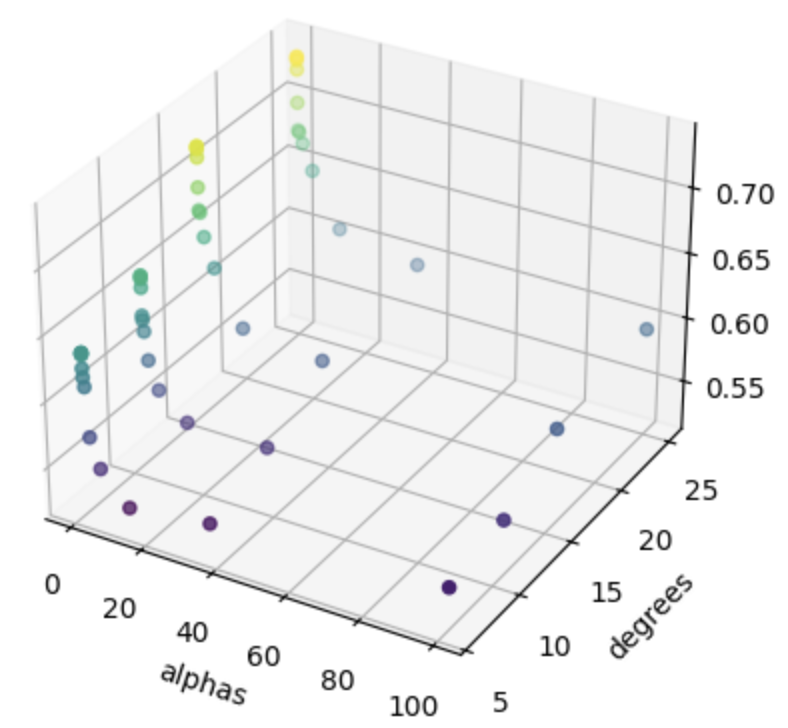
\includegraphics[width=0.75\textwidth]{images/4.png}
	\end{center}
	\caption{Зависимость точности Лассо-регрессии от значения параметра регуляризации и степени полинома}
	\label{img:4}
\end{figure}

\begin{figure}
	\begin{center}
		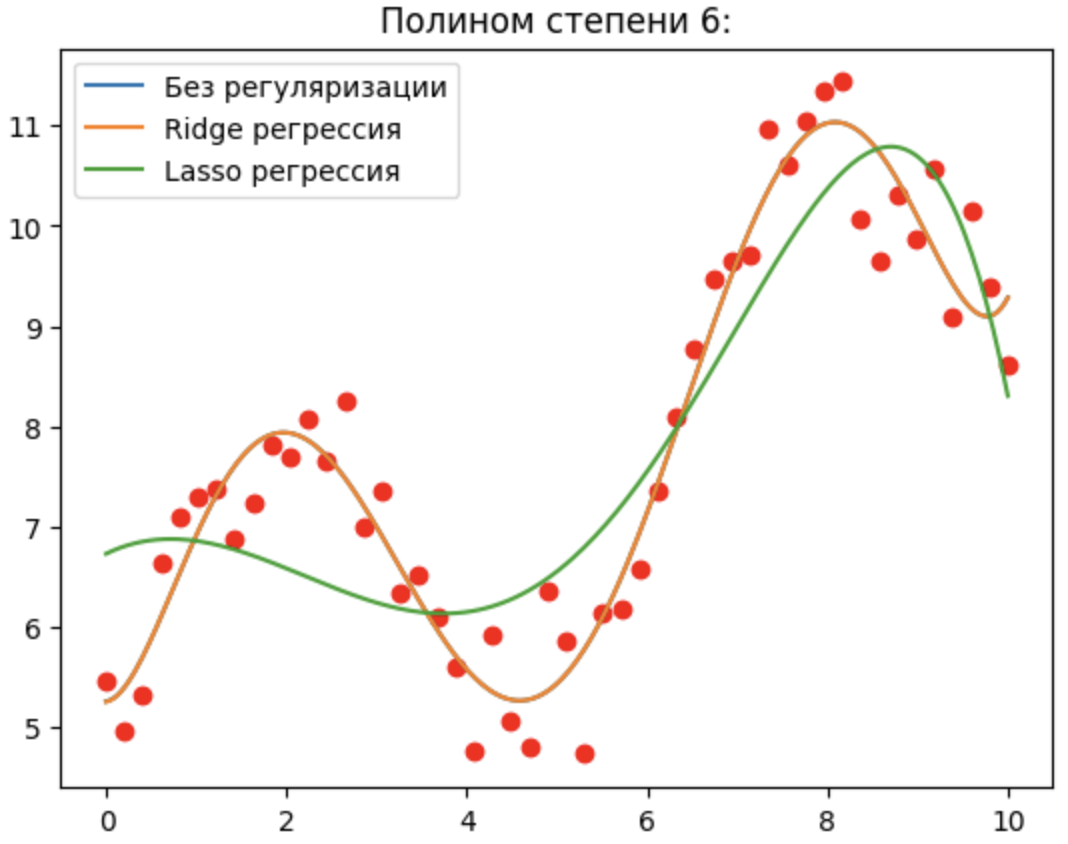
\includegraphics[width=0.75\textwidth]{images/5.png}
	\end{center}
	\caption{Сравнение кривых, полученных без регуляризации, с применением Ридж-регрессии и Лассо-регрессии для полинома степени 6}
	\label{img:5}
\end{figure}

\begin{figure}
	\begin{center}
		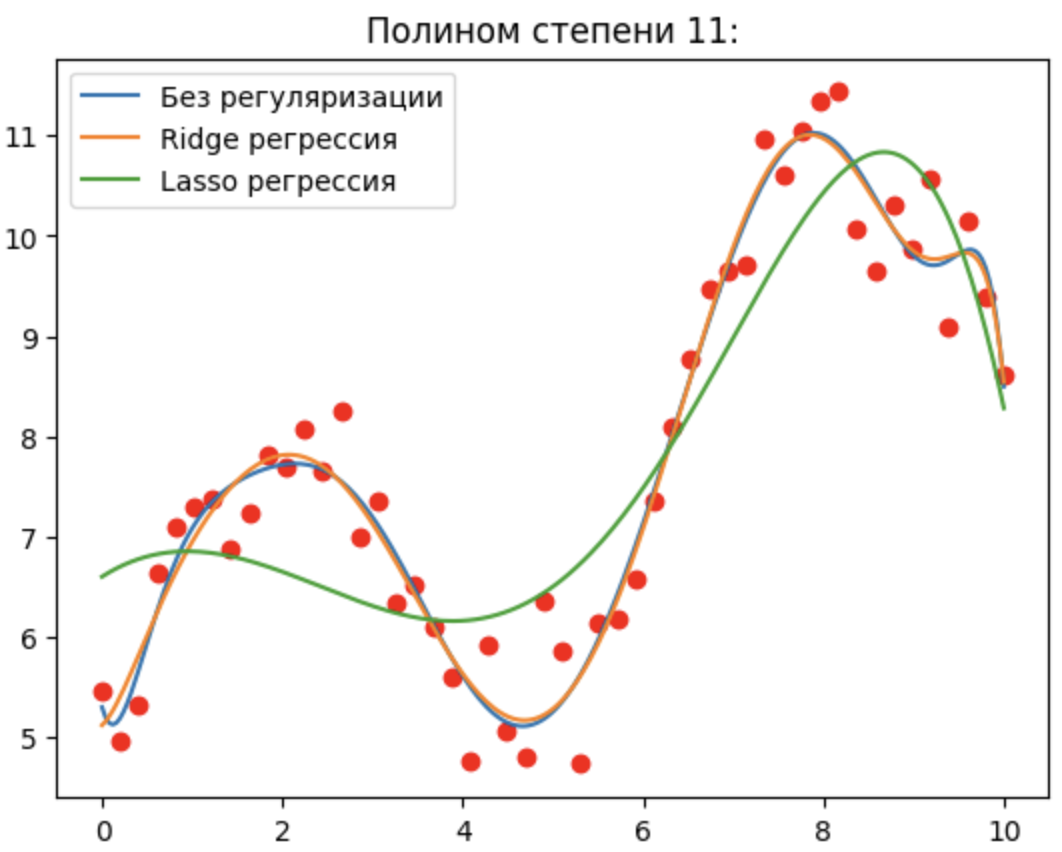
\includegraphics[width=0.75\textwidth]{images/6.png}
	\end{center}
	\caption{Сравнение кривых, полученных без регуляризации, с применением Ридж-регрессии и Лассо-регрессии для полинома степени 11}
	\label{img:6}
\end{figure}

\begin{figure}
	\begin{center}
		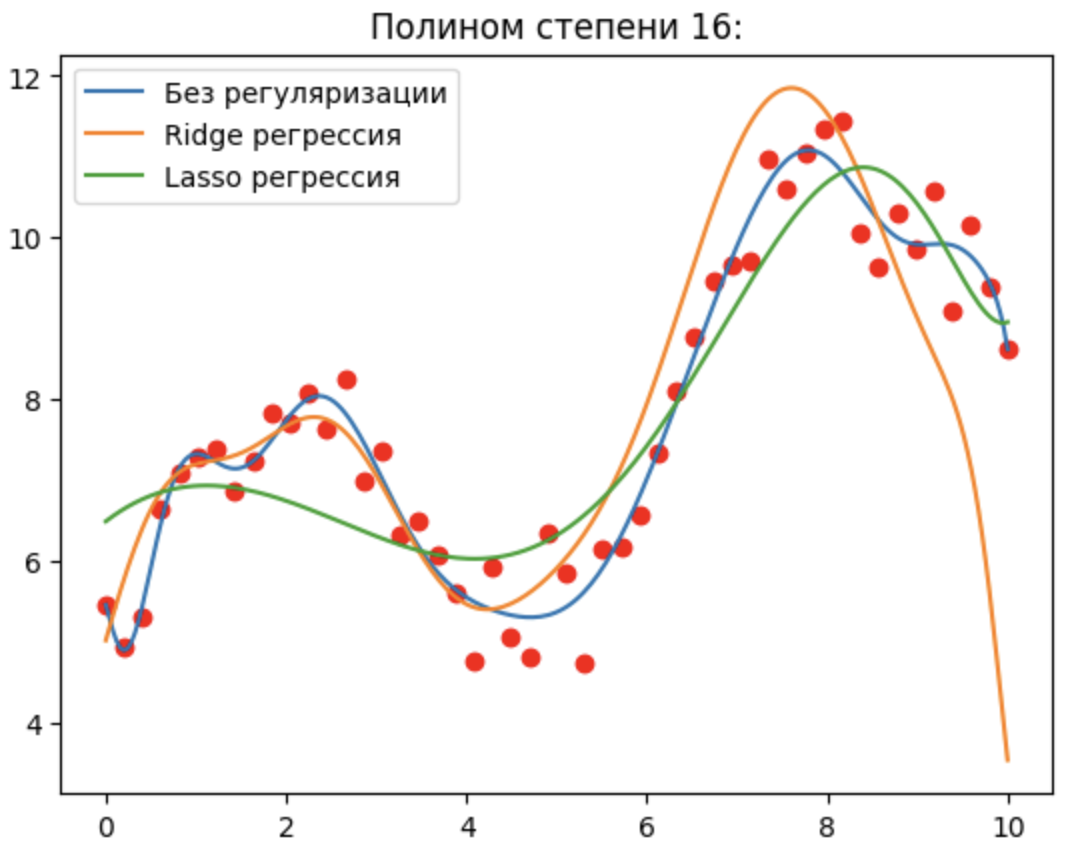
\includegraphics[width=0.75\textwidth]{images/7.png}
	\end{center}
	\caption{Сравнение кривых, полученных без регуляризации, с применением Ридж-регрессии и Лассо-регрессии для полинома степени 16}
	\label{img:7}
\end{figure}

\begin{figure}
	\begin{center}
		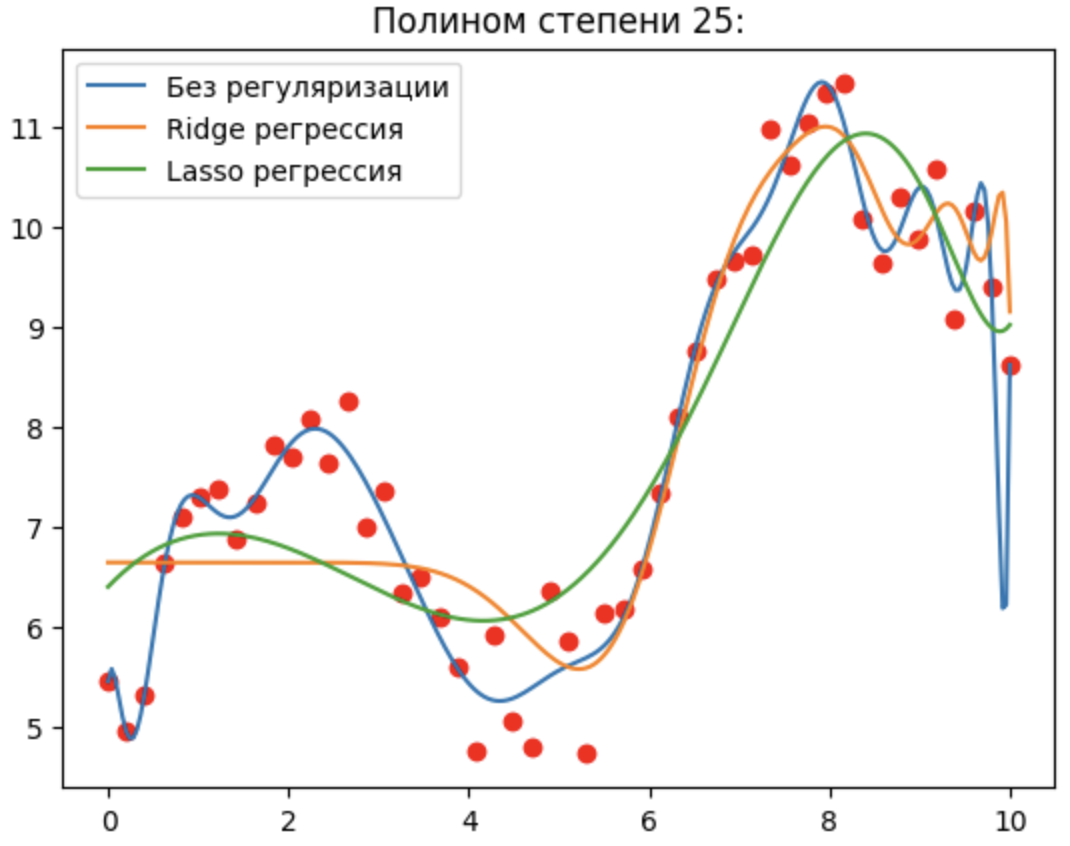
\includegraphics[width=0.75\textwidth]{images/8.png}
	\end{center}
	\caption{Сравнение кривых, полученных без регуляризации, с применением Ридж-регрессии и Лассо-регрессии для полинома степени 25}
	\label{img:8}
\end{figure}

\clearpage
